% !TEX root = ./Basilisk-CoarseSunSensor-20170803.tex

\section{Model Description}

\begin{figure}[htb]
	\centerline{
		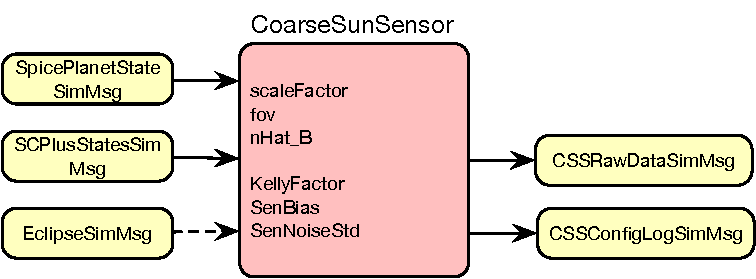
\includegraphics[]{Figures/moduleDiagram}
	}
	\caption{Illustration of the CoarseSunSensor() module I/O}
	\label{fig:moduleDiagram}
\end{figure}
\subsection{Overview}
This document describes how Coarse Sun Sensor (CSS) devices are modeled in the Basilisk software.  Each CSS is modeled through a nominal cosine response relative to the sunlight incidence angle and proportional to light intensity.  It is possible to add individual CSS sensors to the BSK evaluation stack.  However, it is typically simpler to use the {\tt CSSConstellation()} class to store a list of CSS units which are updated as a group, along with a unique CSS array output message.

\subsection{Single CSS module}
\subsubsection{I/O Messages}
First, let us discuss the input and output messages of the individual CSS sensor module.  The two required input messages are of the type {\tt SpicePlanetStateSimMsg} and {\tt SCPlusStatesSimMsg}.  The first message is used to determine the sun's location relative to the inertial frame $\leftexp{N}{\bm r}_{\sun/\mathcal{N}}$.  The second message is used to read in the spacecraft inertial position vector relative to the same inertial frame $\leftexp{N}{\bm r}_{\cal B/N}$.  Finally, the last message is optional.  If it is connected, it provides the sun shadow parameter indicating if the spacecraft is in a planet's shadow.  

The output message of an individual CSS unit creates a message containing the simulated CSS sensor.


\subsubsection{CSS Signal Simulation}
To evaluate the sun heading vector $\bm s$, the satellite and sun position vectors are used.
\begin{equation}
	\leftexp{N}{\bm s} = \leftexp{N}{\bm r}_{\mathrm{Sun}/\mathcal{N}} - \leftexp{N}{\bm r}_{\cal B/N}
\end{equation}
After normalizing this vector to $\hat{\bm s}$ and mapping $\bm\sigma_{\cal B/N}$ to $[BN]$, it is mapped into body frame components through
\begin{equation}
	\leftexp{B}{\hat{\bm s}} = [BN] \leftexp{N}{\hat{\bm s}}
\end{equation}

The CSS sensor unit normal vector is given by $\leftexp{B}{\hat{\bm n}}$ in body frame components.  The normalized cosine sensor signal $\hat\gamma$ is thus determined through
\begin{equation}
	\hat \gamma = \hat{\bm n} \cdot \hat{\bm s} = \cos\phi
\end{equation}
where $\phi$ is the CSS sunlight incidence angle.  
This is the normalized CSS signal where 1 is returned if the sensor is looking straight at the sun.  If the sensor axis $\hat{\bm n}$ is more than the field of view half-angle (set through {\tt fov}) from the sun axis, then a 0 signal is simulated.  This {\tt fov} variable is the angle from $\hat{\bm n}$ beyond which the CSS signal is set to zero.  

The Kelly parameter allows for the CSS signal to pinch towards zero for larger incidence angles as illustrated in Figure~\ref{fig:kelly}.  The amount of signal distortion is set through $\kappa$, where the Kelly factor $p_{\kappa}$ is then computed as 
\begin{equation}
f_{\kappa} = 1 - e^{-\hat\gamma^{2}/\kappa}
\end{equation}
so that the normalized output curve with kelly application is:
\begin{equation}
\gamma_{\kappa} = \gamma f_{\kappa}
\end{equation}
\begin{figure}[htb]
	\centerline{
		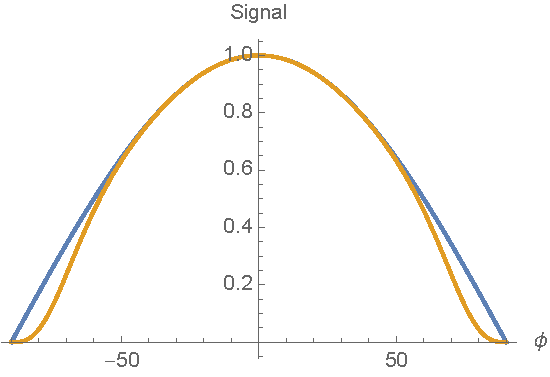
\includegraphics[]{Figures/kelly}
	}
	\caption{Kelly distortion (orange,lower) illustration with $\kappa = 0.1$}
	\label{fig:kelly}
\end{figure}
This reflects the true output behavior of a sun sensor at larger incidence angles. Next, this cosine curve is scaled according to the intensity of the light the sensor receives This includes scaling based on solar flux at a given distance from the sun as well as eclipse shadowing. Note that the model is standardized for 1 AU from the sun so that the output will remain as seen in Fig. \ref{fig:kelly} for an un-eclipsed spacecraft at 1 AU from the sun.
The solar intensity factor based on distance from the sun is:
\begin{equation}
	f_{\mathrm{sunDist}} = \frac{(1 AU)^2}{r_\mathrm{SC/Sun}^2} [\frac{m^2}{m^2}]
\end{equation}
and the shadow factor due to eclipse is given as $f_s$. So the output curve adjusted for light intensity is:
\begin{equation}
	\gamma_{\textrm{li}} = \gamma_{\kappa} f_{\mathrm{sunDist}} f_s 
\end{equation}
If the spacecraft is outside of a planet's shadow, $f_s$ is 1.  If it is within the shadow, then it is $0\le f_{s} < 1$. 
This curve has now accounted for light intensity, but not for the magnitude or units of the sensor electronics output. To do that, a scale factor, $f_{\mathrm{scale}}$ is factored into the equation:
\begin{equation}
	\gamma_{\mathrm{clean}} = f_{\mathrm{scale}} \gamma_{\textrm{li}}
\end{equation}
where $\gamma_{\mathrm{clean}}$ is the output of a sensor with no noise.


Next, Gaussian noise and sensor can be added to the signal The normalized bias is set through {\tt SenBias}, while the normalized noise is set through {\tt SenNoiseStd}.   Let $ n$ be the normalized sensor noise and $b$ be the normalized sensor bias.  Note that these values are non-dimensional and apply to the unscaled output.  Therefore, they will also be scaled when a scale factor is applied to the output. The noisy and appropriately scaled output of the sensor is:
\begin{equation}
	\gamma_{\mathrm{noise}} = (\gamma_{\textrm{li}} + n + b) f_{\mathrm{scale}} 
\end{equation}
This indicates that sensor noise is not a function of light incidence angle or light intensity.
Now, the noise or bias could have caused the sensor to produce a value less than 0 or higher than is possible for the hardware. To prevent this, saturation values are input as and treated as max/min values:
\begin{equation}
	\gamma_{\mathrm{capped}} = \mathrm{min}(\mathrm{maxOutput}, \gamma_{\mathrm{noise}})
\end{equation}
\begin{equation}
	\gamma_{\mathrm{out}} = \gamma_{\mathrm{floored}} = \mathrm{max}(\mathrm{minOutput}, \gamma_{\mathrm{capped}})
\end{equation}
This is the final ouput of the sensor module.




\begin{figure}[htb]
	\centerline{
	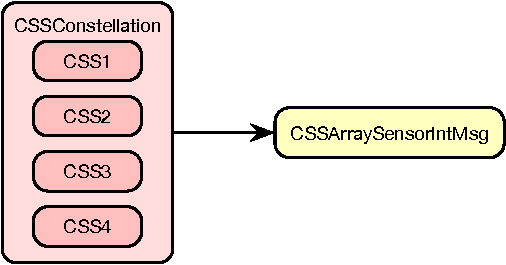
\includegraphics[]{Figures/moduleDiagramConstellation}
	}
	\caption{Illustration of the CSS Constellation class}
	\label{fig:moduleDiagramConstellation}
\end{figure}
\subsection{Constellation or Array of CSS Modules}
The {\tt CSSConstellation} class is defined as a convenience such that the Basilisk update function is called on a group of CSS modules.  Here the CSS BSK modules are created and configured as before, but are then provided to the {\tt CSSConstellation} class object as a list of CSS in python.  The CSS can be configured individually, and must each be connected with the required input messages.  However, the {\tt CSSConstellation} will gather all the CSS outputs and write a single CSS Constellation output message of the type {\tt CSSArraySensorIntMsg} as shown in Figure~\ref{fig:moduleDiagramConstellation}.  



